% !Mode:: "TeX:UTF-8"
\chapter{Introduction}

Nowadays there are many existing image compression approaches. We can divide such algorithms in two groups: lossy (such as JPEG. Mainly such algorithms use Discrete Cosine Transform) and lossless (such as DEFLATE. Mainly such algorithms use similar to Huffman Encoding methods). Both have been developed for decades already. It is important to mention that image containers (such as JPEG, PNG, GIF etc.) are using information compression algorithms \textit{only as a part} of their architecture. Usually lossy and lossless compression methods are combined to achieve higher performance.

Famous JPEG format, for example, has following steps, and only last three are about compression.

\begin{enumerate}
    \item Transformation from RGB to YCbCr (Chroma subsampling).
    \item Quantization. Lossy.
    \item Discrete Cosine Transform. Lossless.
    \item Run-length encoding. Lossless.
    \item Huffman encoding. Lossless.
\end{enumerate}

There is a certain trend to apply a power of neural networks in compression domain, extending a group of lossy algorithms. First approaches were \cite{Balle_Laparra_Simoncelli_2017}, \cite{Theis_Shi_Cunningham_Huszar_2017}, \cite{Toderici_Vincent_Johnston_Hwang_Minnen_Shor_Covell_2017}, where authors proved that it is possible to use one neural network to generate a compressed representation of an image and another neural network to restore initial image from its representation generated by first network. Now such networks are also being used to solve an image and video upscale tasks.

Recent progress in neural image compression has shown a great progress: 

\begin{enumerate}
    \item Now image neural image compression outperform traditional compression algorithms such as JPEG and JPEG2000.
    \item Autoencoder architecture can be extended with different compression modules in between.
    \item Development of convolutional layers architecture provides a more powerful tools to extract image features and reconstruct initial image.
\end{enumerate}

However, several issues are still remaining unsolved:

\begin{enumerate}
    \item False textures.
    \item Limited compression power.
    \item Fixed output size.
\end{enumerate}

We separate neural image compression to two main groups:

\begin{enumerate}
    \item Methods that follow traditional image compression pipeline, while changing some part of it.
    \item Methods that create a new pipeline, while using some parts from traditional pipeline.
\end{enumerate}

For now a general approach is to encode an image to compressed representation using convolutional neural network and take the convolutional features from one of the top layers of network. In this work we are going to use a slightly different architecture.

In this work we are going to apply fully convolutional neural network to extract features from given image, compress those features using another encoder and arithmetic coding algorithm. Then this compressed representation will be restored using decoder and upsample modules. It worth to mention that the algorithm we are working on is lossy. Our method will combine traditional image compression approaches and neural network image compression approach.

\chapter{Objective}

Our motivation is that traditional image compression methods are simple and computationally efficient. However, using more heavy neural models we can compress image much more efficient. By combining these two methods we can reach equilibrium.

Image can be represented using a convolutional features and we can train two neural networks to extract features from given image and reconstruct initial image from these features back. Such a network should have an encoder and a decoder. Encoder is trained to extract meaningful information form given image, which we call feature map or latents; Decoder is trained to reconstruct initial image given latents. We can train such system simply by penalizing L1 or L2 distance between given image and its reconstruction.

\begin{equation}
    \label{eq:1}
    L1=\sum \hat{I}-I
\end{equation}

These intermediate convolutional features already take less disk space than raw initial image. However, we can compress these features using lossless coding algorithm. We are using arithmetic coding because of its huge capacity to compress sequences of numerical values.

It is not difficult to train an autoencoder to compress some information and decompress it back. So, we are using the same design as \cite{Ballé_Minnen_Singh_Hwang_Johnston_2018} to compress hidden features and obtain hyperlatents. Then they can be encoded by lossless compression algorithm.

After compressing image we need to be able to decompress these hyperlatent features back. Say we used lossless coding algorithm to decode hyperlatents, passed them to Hyperprior decoder and get latents. Then we feed these latents to fully convolutional decoder and apply deconvolution operation several times together with upscaling layers to make resulting image bigger. Finally we pass it through several super resolution layers to obtain an image with reduced blur artifacts, more sharp structure and, if needed, higher spacial resolution.

Such a system is complicated and since we need to train it efficiently, we consider using generative adversarial training pipeline to fit the model to data. Discriminator will be trained to till real and generated images apart, which will stabilize training.

\chapter{Niches}

Potentially this work can improve existing image compression algorithms. The disk space required to store hyperlatents is less than disk space required to store raw images or even images encoded with JPEG or JPEG2000. Such an algorithm can be used in different scenarios. Mainly we can use it in traditional use cases for lossy compression such as using it in image format as it is or in more advance sense, to extend existing formats. For example we can extend existing DCT (Discrete Cosine Transform) or DWT (Discrete Wavelet Transform). We selected two possible use cases to apply the compression algorithm we are developing:

\begin{enumerate}
    \item Limited space on machine with high computational power. It can be a big server with powerful CPU. In recent days there are some movements in quantum computing sphere, so it can be a very powerful machine with quantum CPU etc.
    \item Huge images needed to be transmitted through a network with limited speed. In case of a limited performance of a network we can compress and restore images using application, we are working on.
\end{enumerate}

Few years ago already a reasonable performance has been achieved using an encoder-decoder architecture \cite{Theis_Shi_Cunningham_Huszar_2017}. We suppose, that our approach can boost performance both in sense of visual appearance and sense of compressed image size.

The contribution of this work can be considered from two major perspective. The first is that this work is the first approach to use super resolution methods in decoder architecture. From the second perspective we are going to use a general autoencoder architecture together with compression and coding algorithms. And finally our work proposes a new way of thinking of image compression: since we are using fully convolutional neural networks through the whole pipeline of our algorithm, and in decoder we are using upscale layers, user is able to select a size (or scaling factor) of produced images.

\chapter{Methodology}

In our work we compared several approaches to compress images. At first we tried to use a graph as a representation of an image. This approach is quite intuitive, since graph has a certain information about image structure. However, after series of experiments, we figure out that graph cannot represent image identity precisely. And most importantly, current state of the art methods are not capable of producing a good image from a scene graph, since scene graph to image architectures use scene graph to scene layout to image architecture, which makes scene graph a redundant information and only makes reconstructed images worse. We also found out that layout to image algorithms such as \cite{Zhao_Meng_Yin_Sigal_2019} use LSTM network architecture to fuse layout objects into singe representation, but LSTM is not designed to capture spatial relations and fuse objects into single one, since layout objects are unordered. In future this task can be potentially solved by using permutation invariant fusion module.

We use fully convolutional neural networks (FCN) in the encoder \ref{encoder}. FCNs are a family of convolutional neural networks which does not use pooling layers or bilinear interpolation or any other layer that can cause an information loss. Layers like pooling layer only propagate one value though itself. It causes a situation when we cannot determine or learn any information about input to this layer knowing it's output.

Let us consider a pooling layer as an example to make our concern clear. Pooling layer takes a patch from an image (or from a feature map) and aggregates all those values into single output value. Pooling layers usually make use of aggregation functions such as \textit{max}, \textit{min}, \textit{avg} etc. Those functions are permutation invariant, which means we cannot reverse them. Even in theory it is impossible to get an inverse functions for pooling layers kernels, since pooling operation causes information loss.

\begin{figure}[!h]
    \centering
    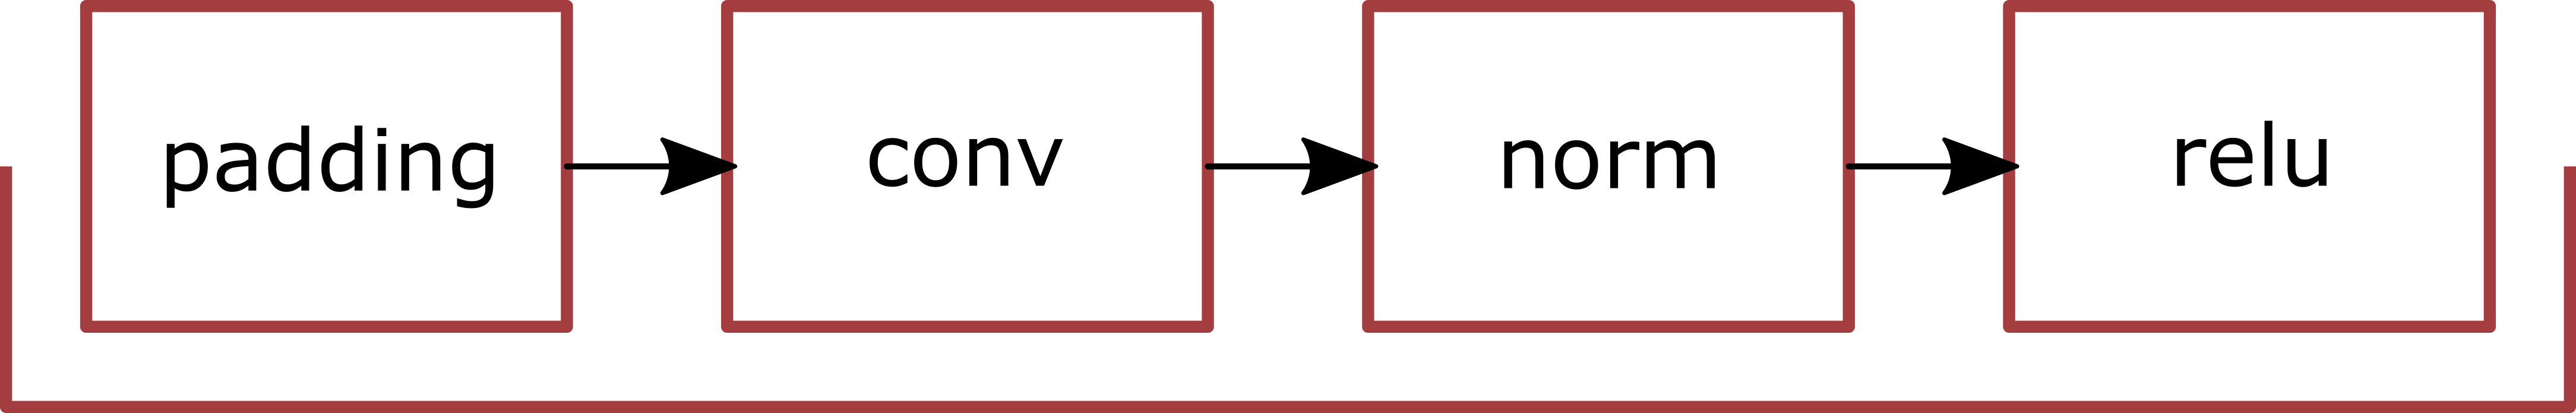
\includegraphics[width=\textwidth]{figure/encoder.png}
    \caption{Convolutional block of the encoder. We stack 6 such blocks to obtain encoder.}
    \label{encoder}
\end{figure}

After a motivation for using FCNs in our encoder, let us take a look on the decoder \ref{decoder}. And the logic here is absolutely same: To restore an image given hidden feature map we need to learn an inverse function, which can be only obtained by reverse of encoder. In practice it means that we need both encoder and decoder to be FCNs \ref{autoencoder}. It will make the entire pipeline less lossy and make an intermediate features more interpretable, since using only convolutional layers helps to achieve a certain consistency in mapping features from input of one layer to its output.

\begin{figure}[!h]
    \centering
    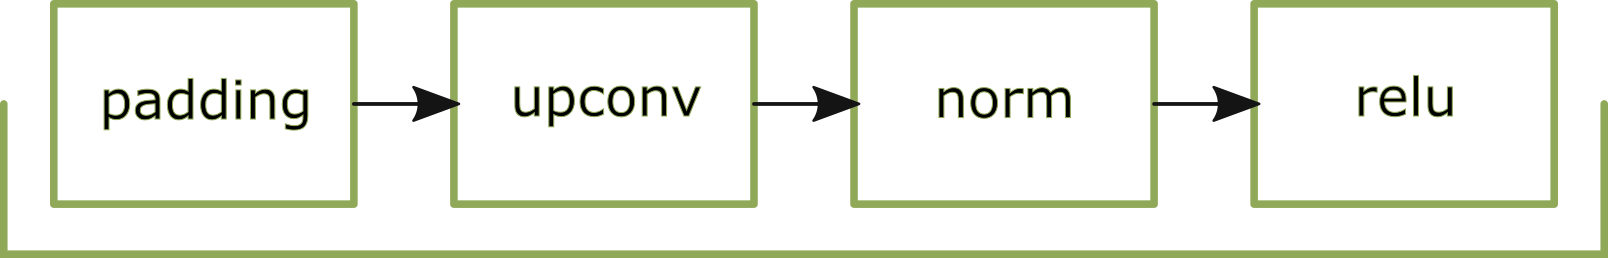
\includegraphics[width=\textwidth]{figure/generator.png}
    \caption{Upconvolutional block (top) and residual block (bottom) of the decoder. We use a combination of these two blocks: We stack 8 residual blocks with 6 upconvolutional blocks on top.}
    \label{decoder}
\end{figure}

We are also using normalization layers in encoder and decoder to make a network more stable. And each convolutional and normalization layer has a residual connection.

\begin{figure}[!h]
    \centering
    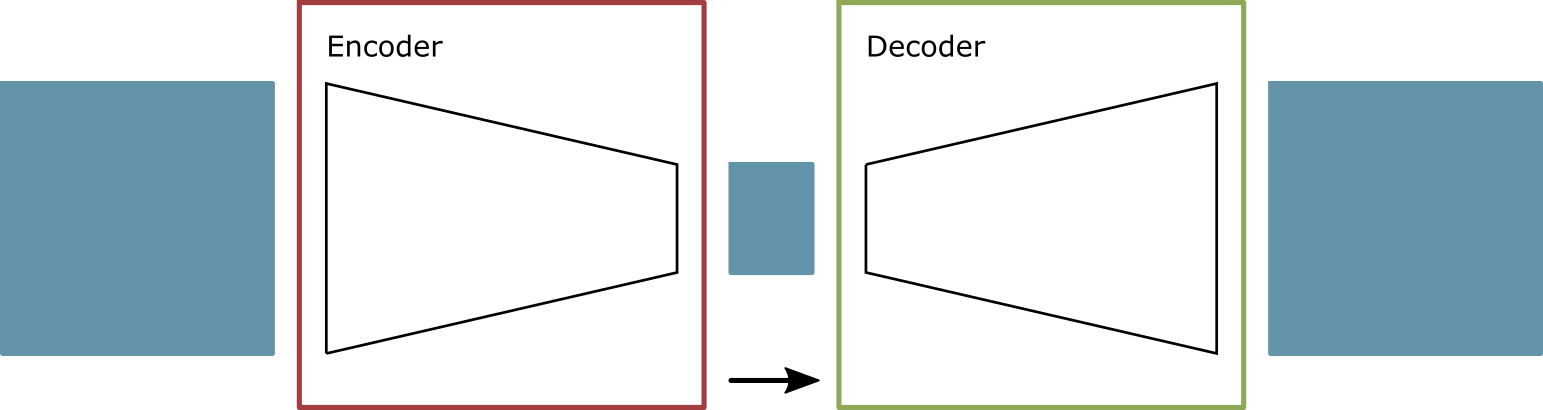
\includegraphics[width=\textwidth]{figure/general-autoencoder.png}
    \caption{Simple autoencoder architecture, which is used in this work. Encoder and decoder are FCNs. Data flow is highlighted to blue. Features in the middle have more channels but less height and width than original image, and this hidden representation takes less space than initial image.}
    \label{autoencoder}
\end{figure}

We can train this autoencoder by minimizing L1 \ref{eq:1} and L2 \ref{eq:2} distance losses. This is a general pipeline for training autoencoder for image compression. Usually other terms are added to the final loss. But even using this simple pipelines we can still reach a reasonable results \ref{autoencoder-result}.

\begin{figure}[!h]
    \centering
    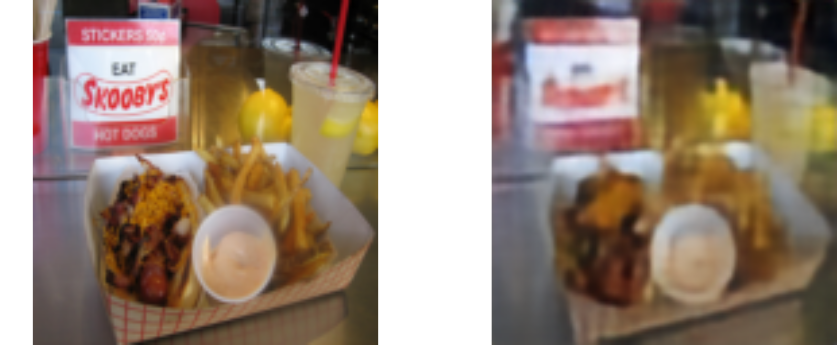
\includegraphics[width=\textwidth]{figure/autoencoder-result.png}
    \caption{Results obtained by training simple autoencoder. (left) Original image, (right) Image obtained after encoding and decoding  using FCN encoder and decoder.}
    \label{autoencoder-result}
\end{figure}

L2 distance loss can be obtained using formula below \ref{eq:2}

\begin{equation}
    \label{eq:2}
    L2=\sum (\hat{I}-I)^2
\end{equation}

Having hidden features (or latents), we can then compress them using one of lossless algorithms such as arithmetic coding or even Huffman coding algorithms. Since we have numerical values here, arithmetic coding is more preferable.

It is possible to use another autoencoder to encode latents obtained from the encoder into hyperlatents, that will have even smaller dimensionality, and apply arithmetic coding to these hyperlatents. We are using a Hyperprior module, which was described in \cite{Ballé_Minnen_Singh_Hwang_Johnston_2018}

\begin{figure}[!h]
    \centering
    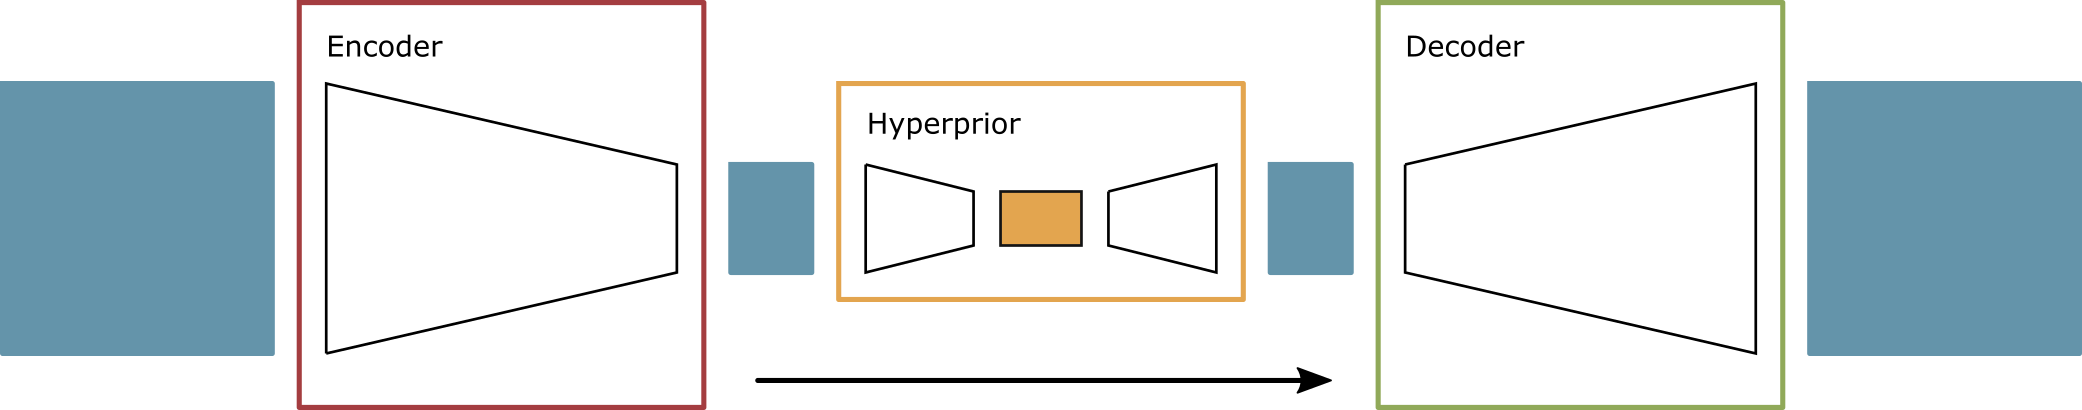
\includegraphics[width=\textwidth]{figure/general.png}
    \caption{Compression general pipeline. Encoder is used to obtain latents, then another encoder is used to obtain hyperlatents. Yellow block is quantization and arithmetic coding block. Then hyperlatents are decoded to latents and the last step is to pass it though Decoder to obtain reconstructed image.}
    \label{whole-system-geneal-pipeline}
\end{figure}

Generative adversarial networks (GANs) show a great performance in training generative models. For GANs training pipeline is slightly different from traditional deep learning pipeline. In \cite{Goodfellow_Pouget-Abadie_Mirza_Xu_Warde-Farley_Ozair_Courville_Bengio_2014} they introduced a neural network training pipeline with two networks: generator and discriminator. Generators objective is to produce a good enough synthetic data. Discriminators objective is to find out, whether given sample synthetic or real. So, trained generator network can be used then to solve a problem.

To train such a system we need two losses: discriminator loss and generator loss. Discriminator loss will penalize discriminator network for it's wrong classification results. The loss we are using in this work is non-saturating loss \ref{eq:loss-g} and \ref{eq:loss-d}, which is just a stable variation of standard GAN loss function. It maximizes the log of the discriminator probabilities.

\begin{equation}
    \label{eq:loss-g}
    \mathcal{L}_G=E_{y\sim p_Y}[-log(D(G(y,s),s))],
\end{equation}

\begin{equation}
    \label{eq:loss-d}
    \mathcal{L}_D=E_{y\sim p_Y}[-log(1-D(G(y,s),s))]+E_{x\sim p_X|s}[-log(D(x,s))]
\end{equation}

The formula above has a following intuition: instead of minimizing a probability of images being fake, it maximizes a probability of images being real, which leads to more stable weight update mechanism.

Since our work is about image compression, we also need to introduce an image compression term in our loss function \ref{eq:loss-eg}. This term is a combination of two values: compression rate loss, which states for a good compression rate of given image and distortion rate, which states for a good quality of reconstructed images. The second term helps to reduce a noise in generated images.

\begin{equation}
    \label{eq:loss-eg}
    \mathcal{L}_{EG}=E_{x\sim p_X}[\lambda r(y)+d(x, x')]
\end{equation}

We can merge \ref{eq:loss-g} an \ref{eq:loss-eg} into one single formula \ref{eq:loss-egp}.

\begin{equation}
    \label{eq:loss-egp}
    \mathcal{L}_{EGP}=E_{x\sim p_X}[\lambda r(y)+d(x, x')-\beta log(D(x',y))]
\end{equation}

So at the end our compression model has two terms, which is exactly the number of terms we want to have while training GAN, since GAN training is performed by incrementally repeating training steps of generator and discriminator. So, we use \ref{eq:loss-egp} during generator train step and we use \ref{eq:loss-d} during discriminator train step.

So, this pipeline describes whole number of actions we need to perform in order to train image compression model. However, images obtained from such model have some unnecessary drawbacks, one of which is the fact that they are blurry \ref{forest-blurry}.

\begin{figure}[!h]
    \centering
    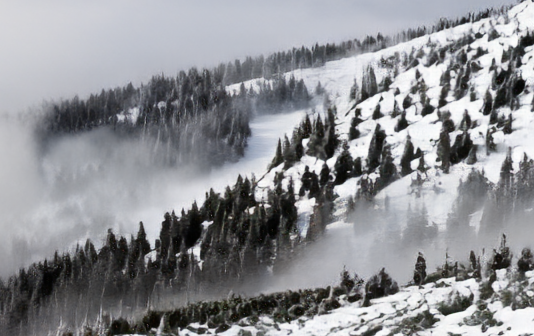
\includegraphics[width=\textwidth]{figure/forest-blurry.png}
    \caption{Example of an image compressed with Hyperprior module.}
    \label{forest-blurry}
\end{figure}

To overcome this issue we propose a novel approach: we include several super resolution layers in our generator. These layers remove blurry artifacts and make resulting images more sharp.

Image super resolution proposal can be formulated as a learning complex degradations from data. It is clear that the first step here is to produce a dataset from that a model then can be learned. Common choice here is to apply degradations on images before passing them into training pipeline.

We consider following degradations: blur, noise, downsampling, JPEG compression. Blur makes image less sharp and here traditional choice is gaussian blur kernel. Noise increases variance of image pixels, common choice is gaussian noise, which is sampled from gaussian distribution. Downsampling operation makes an mage smaller. There are several approaches to resize images: bilinear, bicubic and nearest neighbor interpolation.

For super resolution we use a common architecture, which has been used in \cite{Ledig_Theis_Huszar_Caballero_Cunningham_Acosta_Aitken_Tejani_Totz_Wang_et_al_2017}, \cite{Wang_Yu_Wu_Gu_Liu_Dong_Qiao_Loy_2019}, \cite{Wang_Xie_Dong_Shan_2021}. This architecture also is a fully convolutional net. Here we use a deep convolutional network body to extract meaningful features from an image (this network is 23 layers deep currently). We use residual connections for each layer of the network body. Each residual block performs four convolution operations, having features concatenated with all previous outputs channel-wise \ref{upscale}.

\begin{figure}[!h]
    \centering
    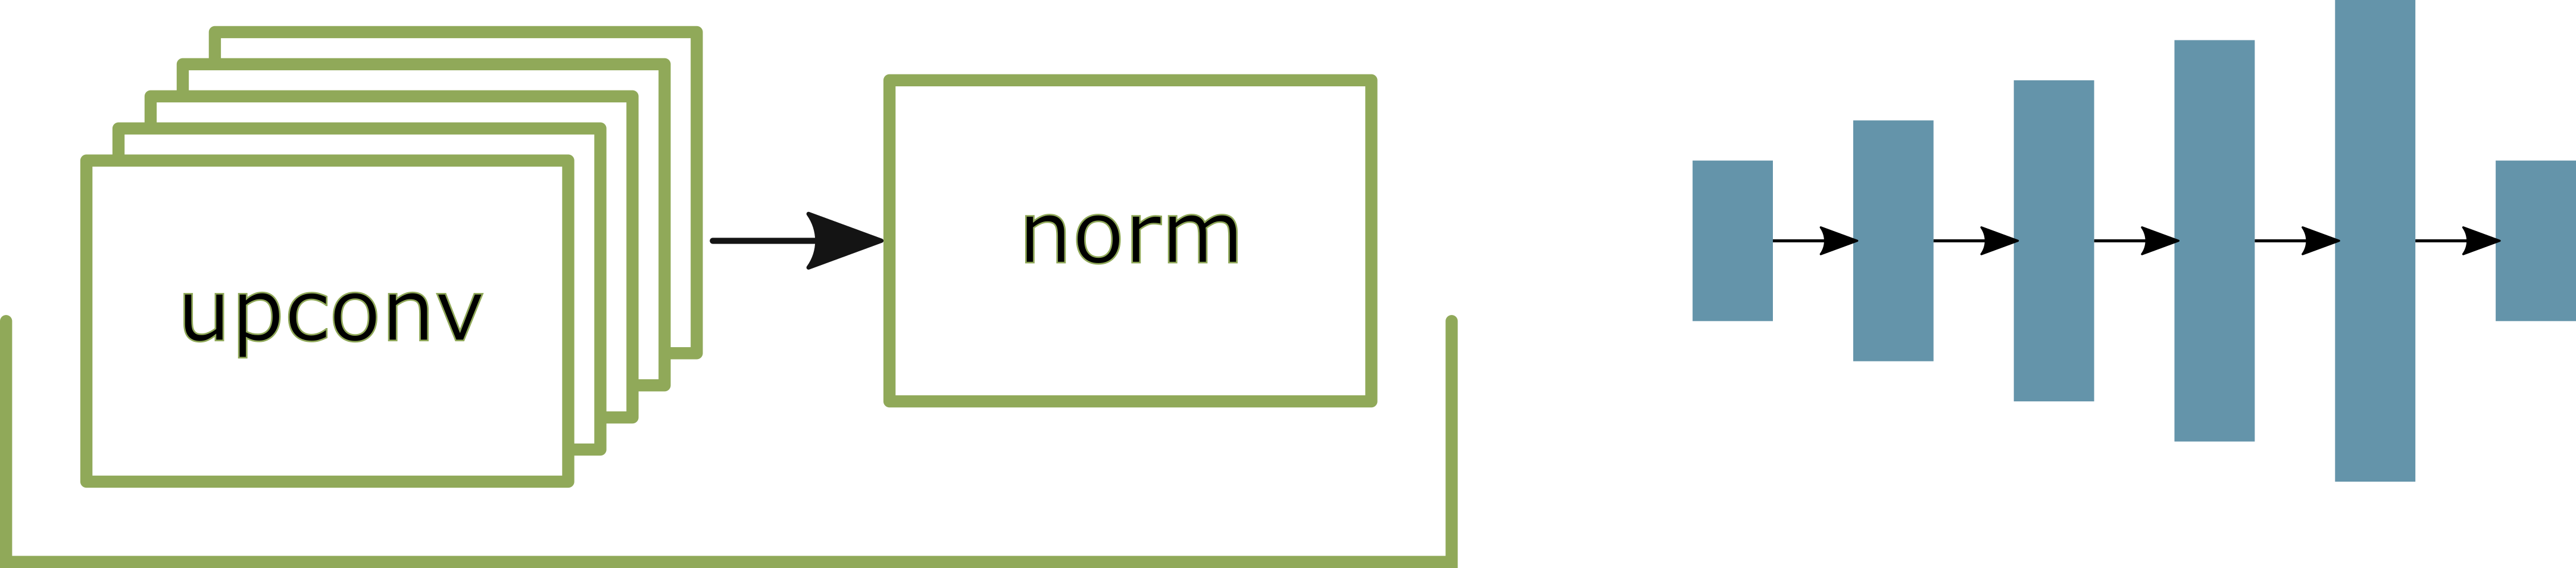
\includegraphics[width=\textwidth]{figure/upscale.png}
    \caption{For upscale we use a combination of convolution layers with residual connection (left). For visualization we also include channel dimensionality dynamics along the propagation through the convolutional layers (right).}
    \label{upscale}
\end{figure}

Having convolutional features propagated through the network body we apply two simple upsampling layers, that use a non-learnable interpolation operation and convolution layer followed by ReLU activation function.

We imply L1 loss \ref{eq:1}, L2 loss \ref{eq:2} and GAN loss \ref{eq:loss-d}, \ref{eq:loss-g} to pretrain super resolution module. Afterwards we fine tune an entire framework. Using same loss functions mentioned above.

\chapter{Experiments}

We train our networks on datasets described in \nameref{section:data}. We set $\lambda$ to $1$ and $\beta$ to $0.15$ parameters from \ref{eq:loss-g}. We set a learning rate of $10^{-4}$ and train the network using Adam optimizer. We train the networks in 2 steps: first step is training compression and upscale networks in GAN manner (using generator and discriminator losses), the second step is to fine tune them together.

\begin{figure}[!h]
    \centering
    \includegraphics[width=\textwidth]{figure/pictures.png}
    \caption{Results of image decompression. Original image is (left), image compressed without upscale module is (middle) and image compressed with upscale module is (right).}
    \label{road}
\end{figure}

By increasing and decreasing $\beta$ and $\lambda$ we can control a tradeoff between compression and distortion loss trams on the training stage. This allows us to select a better hyperparameter for the network. The process of hyperparameter selection is following: start training network and after some number of iterations (we usually wait few epochs) we compare the results of validation dataset. If this set of hyperparameters performs better than previous set, we should use this one. It is clear from \ref{compession-losses}, how compression and distortion losses in combination together give final loss term \ref{eq:loss-egp}.

\begin{figure}[!h]
    \centering
    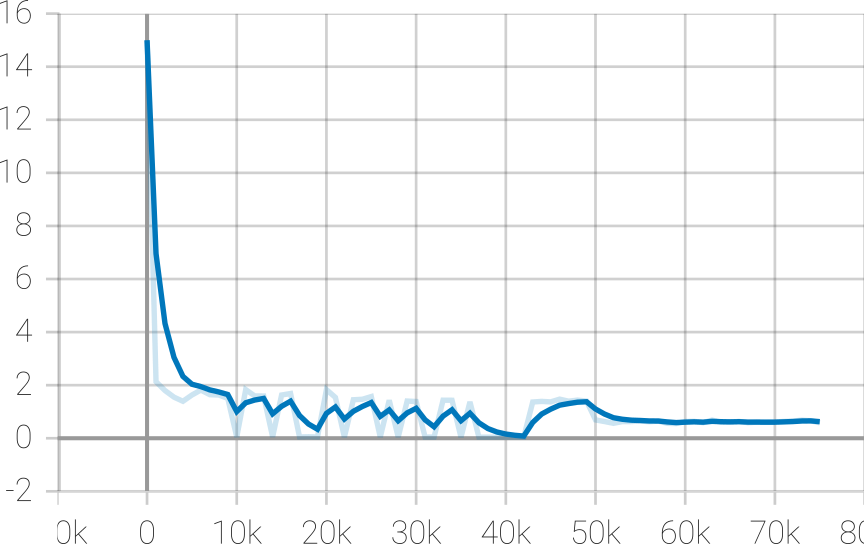
\includegraphics[width=0.3\textwidth]{figure/weighted_compression_weighted_rate.png}
    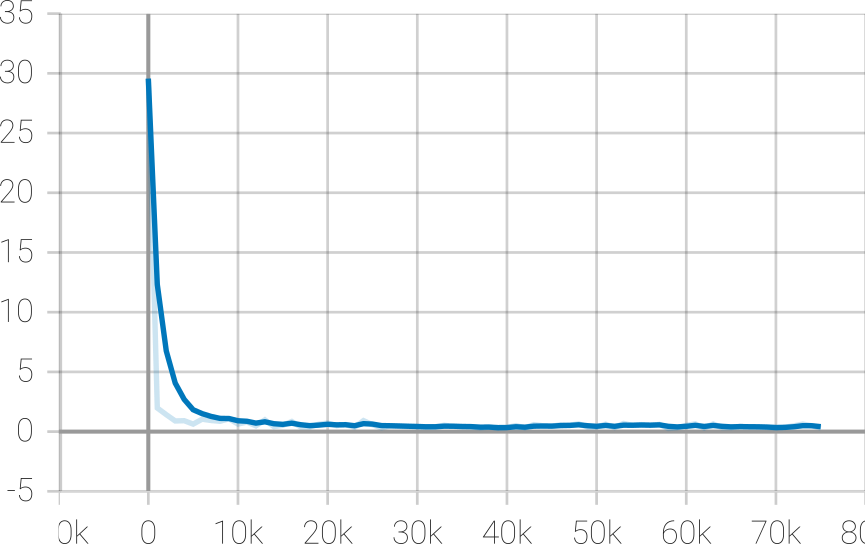
\includegraphics[width=0.3\textwidth]{figure/weighted_compression_weighted_distortion.png}
    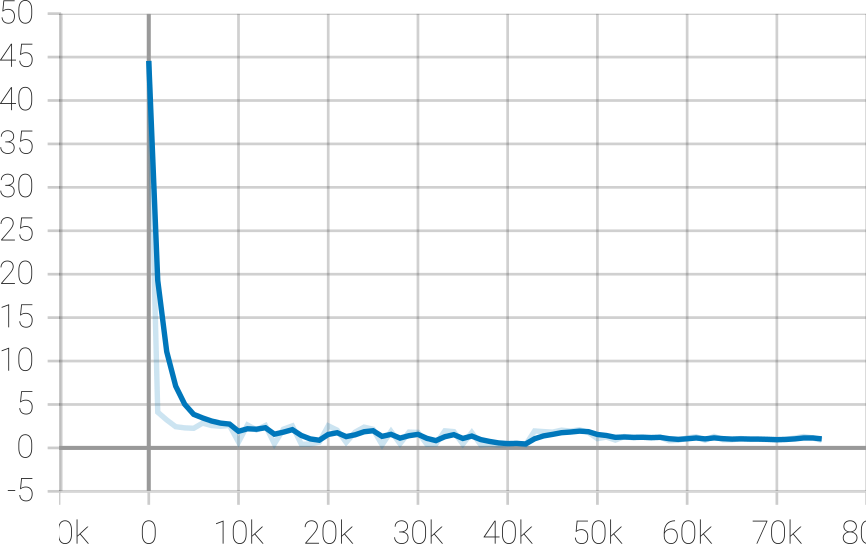
\includegraphics[width=0.3\textwidth]{figure/weighted_compression_weighted_R_D.png}
    \caption{Training process for compression module. As we can see, compression rate term (left) and distortion term (middle) in combination give final rate/distortion loss (right).}
    \label{compession-losses}
\end{figure}

We still do not have enough metric to plot many charts. We figure out, however, that compressed image takes less than 3 times space than JPEG compressed image.

\chapter{Data}
\label{section:data}

We used several datasets to train and test the models we've implemented. One is Visual Genome dataset, which has been used in many other works \cite{Krishna_Zhu_Groth_Johnson_Hata_Kravitz_Chen_Kalantidis_Li_Shamma_etal_2016}. Visual genome consists of more than 100,000 images labeled with scene graphs. We used Visual Genome for training scene graph based compression models.

Dataset consists of several main parts:

\begin{enumerate}
    \item Region descriptions. Human labeled important regions of an image, each description phrase is 1 to 16 words long.
    \item Objects. Objects labeled and canonicalized to a synset ID in WordNet.
    \item Attributes. Both images and objects have attributes. They are also canonicalized to WordNet.
    \item Relationships. Connects a pair of objects. Relationships are directed.
    \item Region graphs. A graph of a region of an image. These could be more than one region graph on one image.
    \item Scene graphs. A composition of region graph of an image. One image has exactly one scene graph.
    \item Question-answer pairs. There are both region-based and freeform QA pairs.
\end{enumerate}

It might be more adequate to split the Visual Genome dataset on the following general parts for better understanding:

\begin{enumerate}
    \item Images in JPEG format with various height and width.
    \item Detected objects information (coordinates of rectangles for each object, objects labels, objects attributes).
    \item Scene graphs, obtained from images.
\end{enumerate}

The dataset itself is quite big (more then 30 Gb), so we implemented a data loader that can work with such amounts of data. There were some efforts \cite{Yang_2018_Graph} to build a framework capable of working with the Visual Genome dataset, however there are no any stable version to work with.

Another dataset we are using in this work is Open Images dataset \cite{OpenImages2}, which is a a huge dataset of 9 million images. Those images are annotated with image-level and object-level annotations, bounding boxes, visual relations and segmentation masks. We use this dataset to train and test models of image compression, which means we do only need clean images without annotations. We use near 150,000 images subset from 9,000,000 images dataset. This amount is sufficient to train a compression model.

\chapter{Future work}

Future work mainly incudes improvements of Generator network. We plan to reduce number of layers in generator by applying the same backbone network to both upscale and deconvolution networks. This will help to reduce a number of training and fine tuning iterations and help to reduce number of parameters, which will directly affect portability of the network to devices with small GPU. We also think that by improving a backbone we can increase an accuracy of reconstructions and resolve a false textures issue, but it still needs to be tested.

There also is an issue with metics for this work. For the final thesis we need to collect metics that will reflect three aspects of our complex network:

\begin{enumerate}
    \item Compression ratio. We plan to use traditional BPP (bits pe pixel) metic, since this number can show the effectiveness of compression.
    \item Reconstructed image distortion. We plan to use a distance between images for this metric. In combination with PSNR (pike signal to noise ratio) it can reflect similarity between original and reconstructed image.
    \item Upscale image quality. Since we also include upscale layers, it's important to measure a quality of upscale images. Unfortunately, it is not possible to directly measure, how good upscale operation performs, however we consider traditional tick, such as downsizing initial image before training.
\end{enumerate}

\chapter{Schedule and arrangement}

Proposed architecture has a compound structure. As it has been mentioned above, the architecture can be separated into two major parts: encoder and decoder part. From our experiments we see that encoder part performs good and there is no need to improve it. However, decoder part is a bit too heavy and complicated. We plan to improve it and reduce number of parameters.

We refer to the schedule from thesis proposal \ref{tab:schedule}.

\begin{table}
    \centering
    \caption{Schedule}
    \label{tab:schedule}
    \begin{tabular}{p{4cm}|p{8cm}|p{2cm}|p{2cm}}
        \hline
        Task & Description & Deadline & Status \\
        \hline
        Build a model prototype & Build a first version of a model that is capable to compress and restore images, it will include building and training encoder and decoder & September 1 & Done \\
        \hline
        Improve model prototype & Adjust parameters, decide on additional convolutional features size & December 1 & Done \\
        \hline
        Research proposal 1 & Reduce number of layers in generator & February 1 & In progress \\
        \hline
        Research proposal 2 & Solve false textures issue & March 1 & In progress \\
        \hline
        Write the final thesis & Summarize research in the final thesis & May 20 & In progress \\
        \hline
    \end{tabular}
\end{table}

Tasks in this table are not really concrete. So it's more like a template for future planning. We are using Trello software to deal with concrete short-term tasks. Time management however is not a part of a technical part of the project, so we just mention it here.